\documentclass{article}
\usepackage{amsmath, amssymb, amsfonts, amsthm, mathtools, bm}
\usepackage{geometry}
\usepackage{hyperref}
\usepackage[english]{babel}
\usepackage{graphicx}

\title{Blending SIR and Predator-Prey Models to Predict the Labor Market}

\author{Jason Vasquez \and Dylan Skinner \and Benjamin Mcmullin \and Ethan Crawford}

\date{December 5 2023}

\begin{document}

\maketitle

We give permission for this work to be shared by ACME Volume 4 instructors and anybody else who may have reasonable motivation.

\begin{abstract}

The labor market, including the unemployment rate and the amount of workers looking for jobs, can have a large impact on the economny.
The more people employed means more money being spent, which in turn means more money being made. 
Furthermore, rise in unemployment can lead to a recession. Being able to predict the labor market can help us prepare for a recession and help us understand the economy better.
In this paper, we adapt an SIR model to model the amount of employed, unemployed, and retired individuals.
Furthermore, we use a quasi predator-prey model to illustrate the oscillation of the two industries commonly known as white-collar and blue-collar.

\end{abstract}

\section{Background/Motivation}


Our investigation navigates the intricate dynamics of employment trajectories and occupational sectors. 
Employing the SIR (Susceptible-Infectious-Recovered) model, typically used for disease dynamics but adapted 
here to study employment dynamics, we aim to comprehend the propagation of employment statuses—specifically, 
the transitions between being employed, unemployed, and retired. A discernible trend has emerged in recent times, 
notably influenced by the technological revolution. The surge in interest and demand for tech-oriented careers 
has prompted a significant shift away from traditional blue-collar professions. This migration has led to a 
dual challenge: a scarcity of skilled workers in the blue-collar sector and an oversaturation of the tech 
industry. Our study extends beyond the conventional SIR model, incorporating elements of a quasi-predator-prey 
framework inspired by ecological models. This approach allows us to capture the nuanced relationship between 
the blue-collar and white-collar industries, offering insights into the cyclical dynamics between these sectors. 
Motivated by the imperative to comprehend and address the consequences of this evolving employment landscape, 
our research aims to contribute valuable insights for informing strategic policies and industry interventions.

\subsection{Related Work}

Here is a cool graph. Please accept it as nothing but the truth.

\begin{figure}[h]
    \centering
    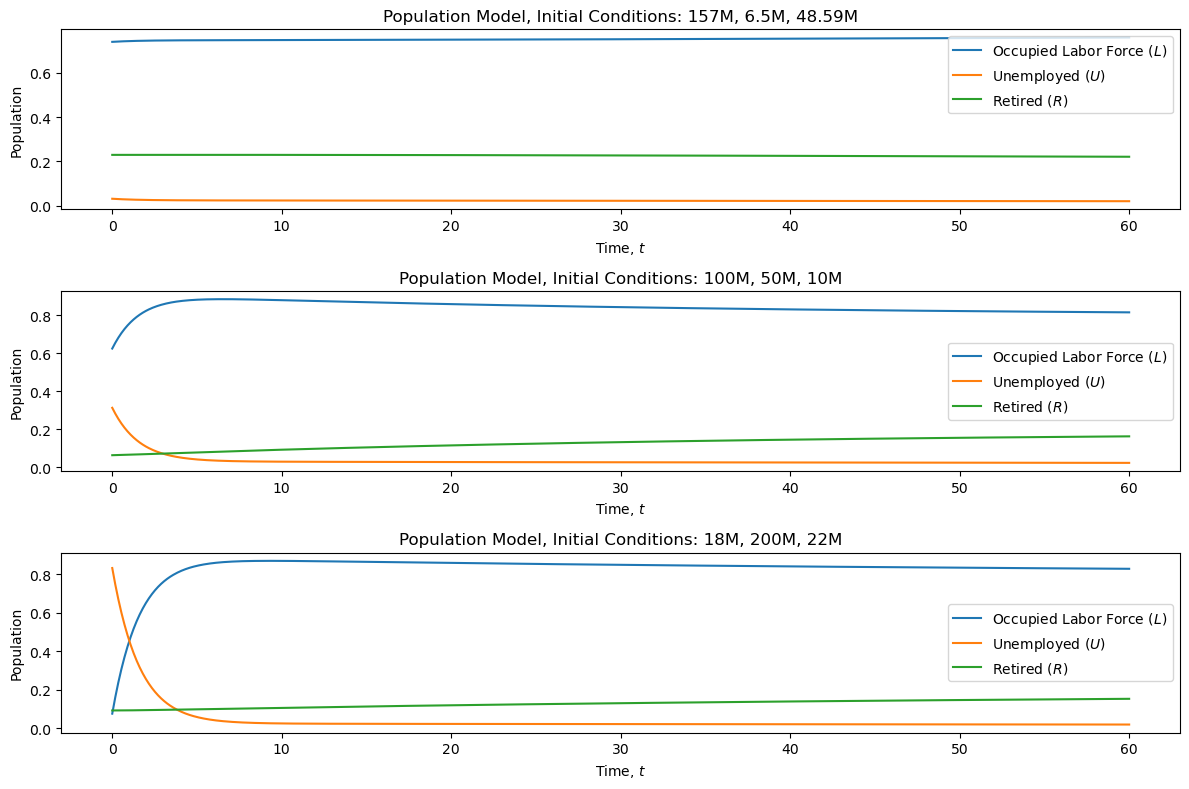
\includegraphics[width=\textwidth]{figures/vol4_proj_pic.png}
    \caption{A cool graph}
    \label{fig:cool_graph}
\end{figure}

% Rest of your document goes here

\end{document}
